\documentclass{article}
\usepackage{graphicx} % Required for inserting images
\usepackage{amsmath}
\usepackage{amsfonts}
\usepackage{comment}
\usepackage{microtype}
\usepackage{bm}
\usepackage{multicol}

\usepackage{mathtools}
\DeclarePairedDelimiter\bra{\langle}{\rvert}
\DeclarePairedDelimiter\ket{\lvert}{\rangle}
\DeclarePairedDelimiterX\braket[2]{\langle}{\rangle}{#1\delimsize\vert\mathopen{}#2}
\newcommand*\diff{\mathop{}\!\mathrm{d}}
\DeclarePairedDelimiterX\expval[3]{\langle}{\rangle}%
{#1\delimsize\vert\mathopen{}#2\delimsize\vert\mathopen{}#3}
\newcommand\HF{\ensuremath{\mathrm{HF}}}

\usepackage{hyperref}
\usepackage{xcolor}
\hypersetup{ % this is just my personal choice, feel free to change things
    colorlinks,
    linkcolor={red!50!black},
    citecolor={blue!50!black},
    urlcolor={blue!80!black},
}

\usepackage{simpler-wick}

\usepackage{enumerate}
\usepackage[shortlabels]{enumitem}
\usepackage{booktabs}

\renewcommand\thesection{Part \alph{section})}  % chktex 9 % chktex 10 % tex-fmt: skip
\renewcommand\thesubsection{Solution} % tex-fmt: skip
\renewcommand\thesubsubsection{\arabic{subsection}.\arabic{subsubsection})} % chktex 9 % chktex 10 % tex-fmt: skip

\title{
    First midterm FYS4480\\
    Quantum mechanics for many-particle systems
}
\author{August Femtehjell \& Oskar Idland}
\date{October 2024}

\begin{document}

\maketitle

\section*{Introduction}

In this midterm we will develop two simple models for studying the helium atom (with two electrons) and the beryllium atom with four electrons.

After having introduced the  Born-Oppenheimer approximation which effectively freezes out the nucleonic degrees of freedom, the Hamiltonian for \(N\) electrons takes the following form
\begin{equation*}
    \hat{H} = \sum_{i=1}^{N} t(x_i) - \sum_{i=1}^{N} k\frac{Ze^2}{r_i} + \sum_{i<j}^{N} \frac{ke^2}{r_{ij}},
\end{equation*}
with \(k=1.44\) eVnm.
Throughout this work we will use atomic units, this means that \(\hbar = c = e = m_e = 1\).
The constant \(k\) becomes also equal 1.
The resulting energies have to be multiplied by \(2 \times 13.6\) eV in order to obtain energies in eletronvolts.

We can rewrite our Hamiltonians as
\begin{equation}
    \hat{H} = \hat{H_0} + \hat{H_I}
    = \sum_{i=1}^{N}\hat{h}_0(x_i) + \sum_{i<j}^{N}\frac{1}{r_{ij}},
    \label{eq:H1H2}
\end{equation}
where  we have defined \(r_{ij} = |\boldsymbol{r}_i - \boldsymbol{r}_j|\) and \(\hat{h}_0(x_i) =  \hat{t}(x_i) - \frac{Z}{r_i}\).

The variable \(x\) contains both the spatial coordinates and the spin values.
The first term of Eq.~\eqref{eq:H1H2}, \(H_0\), is the sum of the \(N\) \emph{one-body} Hamiltonians \(\hat{h}_0\).
Each individual Hamiltonian \(\hat{h}_0\) contains the kinetic energy operator of an electron and its potential energy due to the attraction of the nucleus.
The second term, \(H_I\), is the sum of the \(N(N-1)/2\) two-body interactions between each pair of electrons.
Note that the double sum carries a restriction \(i<j\).

As basis functions for our calculations we will use hydrogen-like single-particle functions.
This means the onebody operator is diagonal in this basis for states \(i,j\) with quantum numbers
\(n,l,m_l,s,m_s\) with energies
\begin{equation}
    \expval{i}{\hat{h}_0}{j} = -\frac{Z^2}{2n^2}\delta_{ij}.
    \label{eq:onebody}
\end{equation}
The quantum number \(n\) refers to the number of nodes of the wave function.
Observe that this expectation value is independent of spin.

We will in all calculations here restrict ourselves to only so-called \(s\)-waves, that is the orbital momentum \(l\) is zero.
We will also limit the quantum number \(n\) to \(n \le 3\).
It means that every \(ns\) state can accommodate two electrons due to the spin degeneracy.

In the calculations you will need the Coulomb interaction with matrix elements involving single-particle wave functions with \(l = 0\) only, the
so-called \(s\)-waves.
We need only the radial part since the spherical harmonics for the \(s\)-waves are rather simple.
We omit single-particle states with \(l > 0\).
The actual integrals we need, are tabulated at the end.
Our radial wave functions are
\begin{equation*}
    R_{n0}(r) = \left( \frac{2Z}{n} \right)^{3/2} \sqrt{\frac{(n-1)!}{2n\times n!}} L_{n-1}^1 \left( \frac{2Zr}{n} \right) \exp{\left( -\frac{Zr}{n} \right)},
\end{equation*}
where \(L_{n-1}^1(r)\) are the so-called Laguerre polynomials.
These wave functions can then be used to compute the direct part of the Coulomb interaction
\begin{equation*}
    \expval*{\alpha\beta}{V}{\gamma\delta} = \int r_1^2 dr_1 \int r_2^2 dr_2 R_{n_{\alpha} 0}^*(r_1) R_{n_{\beta} 0}^*(r_2) \frac{1}{r_{12}}R_{n_{\gamma} 0}(r_1) R_{n_{\delta} 0}(r_2).
\end{equation*}

Observe that this is only the radial integral and that the labels \( \alpha,\beta,\gamma,\delta \) refer only to the quantum numbers \(n,l,m_l\), with \(m_l\) the projection of the orbital momentum \(l\).
A similar expression can be found for the exchange part.
Since we have restricted ourselves to only \(s\)-waves, these integrals are straightforward but tedious to calculate.
As an addendum to this midterm we list all closed-form expressions for the relevant matrix elements.
Note well that these matrix elements do not include spin.
When setting up the final antisymmetrized matrix elements you need to consider the spin degrees of freedom as well.
Please pay in particular attention to the exchange part and the pertinent spin values of the single-particle states.

We will also, for both helium and beryllium assume that the many-particle states we construct have always the same total spin projection \(M_S = 0\).
This means that if we excite one or two particles from the ground state, the spins of the various single-particle states should always sum up to zero.

\section{Setting up the basis}
We start with the helium atom and define our single-particle Hilbert
space to consist of the single-particle orbits \(1s\), \(2s\) and \(3s\),
with their corresponding spin degeneracies.

Set up the ansatz for the ground state \(\ket*{c} = \ket*{\Phi_0}\) in second quantization.
Define the second quantization and define a table of single-particle states.
Construct thereafter all possible one-particle-one-hole
excitations \(\ket*{\Phi_i^a}\) where \(i\) refer to levels below the Fermi level (define this level) and \(a\) refers to particle states.
Define particles and holes.
The Slater determinants have to be written in terms of the respective creation and annihilation operators.
The states you construct should all have total spin projection \(M_S=0\).
Construct also all possible two-particle-two-hole states \(\ket*{\Phi_{ij}^{ab}}\) in a second quantization
representation.

\subsection{}
We define the Fermi level as \(1s\), such that the ground state is given by
\begin{equation}
    \ket*{\Phi_0} = \ket*{c} = a_{1\sigma_1}^\dagger a_{1\sigma_2}^\dagger \ket*{0},
\end{equation}
where we define $\sigma_1 = \ \uparrow \ = +1/2$ and $\sigma_2 = \ \downarrow \ = -1/2$.
Here, we define particles as electrons (?) above the Fermi level, and holes as the lack of electrons in slots below the Fermi level.

In order to have a one-particle-one-hole excitation, the spin in the hole and particle states must match.
All possible one-particle-one-hole (1p1h) excitations are then
\begin{align*}
    \ket*{\Phi_{1\sigma_1}^{2\sigma_1}} &= a_{2\sigma_1}^\dagger a_{1\sigma_1} \ket*{\Phi_0}, &
    \ket*{\Phi_{1\sigma_1}^{3\sigma_1}} &= a_{3\sigma_1}^\dagger a_{1\sigma_1} \ket*{\Phi_0}, \\
    \ket*{\Phi_{1\sigma_2}^{2\sigma_2}} &= a_{2\sigma_2}^\dagger a_{1\sigma_2} \ket*{\Phi_0}, &
    \ket*{\Phi_{1\sigma_2}^{3\sigma_2}} &= a_{3\sigma_2}^\dagger a_{1\sigma_2} \ket*{\Phi_0},
\end{align*}
where we always excite a particle from the $1s$ state, to the higher states, with the same spin such that $M_S = 0$.

For the possible two-particle-two-hole (2p2h) excitations $\ket*{\Phi_{ij}^{ab}}$, we have that both electrons below the Fermi level excite, and that the particles above the Fermi level have opposite spins.
We then have that the possible configurations are
\begin{align*}
    \ket*{\Phi_{1\sigma_1, 1\sigma_2}^{2\sigma_1, 2\sigma_2}} &= a_{2\sigma_1}^\dagger a_{2\sigma_2}^\dagger a_{1\sigma_2} a_{1\sigma_1} \ket*{\Phi_0}, &
    \ket*{\Phi_{1\sigma_1, 1\sigma_2}^{2\sigma_1, 3\sigma_2}} &= a_{2\sigma_1}^\dagger a_{3\sigma_2}^\dagger a_{1\sigma_2} a_{1\sigma_1} \ket*{\Phi_0}, \\
    \ket*{\Phi_{1\sigma_1, 1\sigma_2}^{3\sigma_1, 2\sigma_2}} &= a_{3\sigma_1}^\dagger a_{2\sigma_2}^\dagger a_{1\sigma_2} a_{1\sigma_1} \ket*{\Phi_0}, &
    \ket*{\Phi_{1\sigma_1, 1\sigma_2}^{3\sigma_1, 3\sigma_2}} &= a_{3\sigma_1}^\dagger a_{3\sigma_2}^\dagger a_{1\sigma_2} a_{1\sigma_1} \ket*{\Phi_0}.
\end{align*}



\section{Second quantized Hamiltonian}
% Define the Hamiltonian in a second-quantized form and use this to compute the expectation value of the ground state (defining the so-called reference energy and later our Hartree-Fock functional) of
the helium atom.
Show that it is given by
\begin{equation}
    E[\Phi_0] = \expval{c}{\hat{H}}{c} = \sum_{i} \expval{i}{\hat{h}_0}{i} + \frac{1}{2} \sum_{ij} \left[\expval*{ij}{\frac{1}{r_{ij}}}{ij} - \expval*{ij}{\frac{1}{r_{ij}}}{ji}\right].
\end{equation}
Define properly the sums keeping in mind that the states $ij$ refer to all quantum numbers $n, l, m_l, s, m_s$.
Use the values for the various matrix elements listed at the end of the midterm to find the value of $E$ as function of $Z$ and compute $E$ as function of $Z$.

\subsection{}
We consider the Hamiltonian $\hat{H} = \hat{H}_0 + \hat{H}_I$, where $\hat{H}_0$ is the one-body part and $\hat{H}_I$ is the two-body part, given by
\begin{align*}
    \hat{H}_0 &= \sum_{i=1}^{N}\hat{h}_0(x_i), &
    \hat{H}_I &= \sum_{i<j}^{N}\frac{1}{r_{ij}}.
\end{align*}
In second quantization, we rewrite the one-body part as
\begin{equation}
    \hat{H}_0 = \sum_{\alpha\beta} \expval{\alpha}{\hat{h}_0}{\beta} a_\alpha^\dagger a_\beta.
\end{equation}
With the new annihilation and creation operators $b_\alpha$ and $b_\alpha^\dagger$ with respect to the new vacuum state $\ket*{\Phi_0}$, we can rewrite this as
\begin{equation}\label{eq:H0_second_quant}
    \begin{split}
        \hat{H}_0 =& \sum_{ab} \expval{a}{\hat{h}_0}{b} b_a^\dagger b_b + \sum_{ai} \left[ \expval{a}{\hat{h}_0}{i} b_a^\dagger b_i^\dagger + \expval{i}{\hat{h}_0}{a} b_i b_a \right] \\
        &+ \sum_{i} \expval{i}{\hat{h}_0}{i} - \sum_{ij} \expval{j}{\hat{h}_0}{i} b_i^\dagger b_j.
    \end{split}
\end{equation}

Recalling that
\begin{equation*}
    \expval{\alpha}{\hat{h}_0}{\beta} = -\frac{Z^2}{2n^2}\delta_{\alpha \beta},
\end{equation*}
we can simplify the expression to
\begin{equation}\label{eq:H0_second_quant_simple}
    \hat{H}_0 = \sum_{a} \expval{a}{\hat{h}_0}{a} b_a^\dagger b_a + \sum_{i} \expval{i}{\hat{h}_0}{i} - \sum_{i} \expval{i}{\hat{h}_0}{i} b_i^\dagger b_i.
\end{equation}
The first and last terms vanish, as both $b_\alpha \ket*{\Phi_0} = 0$, leaving us with
\begin{equation}
    \expval{c}{\hat{H}_0}{c} = \sum_{i} \expval{i}{\hat{h}_0}{i} \braket{c}{c} =: \mathcal{E}_0^{\text{Ref}}.
\end{equation}

The two-body part is rewritten in second quantization as
\begin{equation}
    \hat{H}_I = \frac{1}{2} \sum_{\alpha \beta \gamma \delta} \expval{\alpha \beta}{V}{\gamma \delta} a_\alpha^\dagger a_\beta^\dagger a_\delta a_\gamma.
\end{equation}
With the new annihilation and creation operators, we can rewrite this as
\begin{equation*}
    \hat{H}_I = \hat{H}_I^{(1)} + \hat{H}_I^{(2)} + \hat{H}_I^{(3)} + \hat{H}_I^{(4)} + \hat{H}_I^{(5)},
\end{equation*}
where utilizing antisymmetrized matrix elements for the sake of brevity, we have
\begin{align*}
    \hat{H}_I^{(1)} &= \frac{1}{4} \sum_{abcd} \expval{ab}{V}{cd} b_a^\dagger b_b^\dagger b_d b_c, \\
    \hat{H}_I^{(2)} &= \frac{1}{4} \sum_{abci} \expval{ab}{V}{ci} b_a^\dagger b_b^\dagger b_i^\dagger b_c + \expval{ai}{V}{cb} b_a^\dagger b_i b_b b_c \\
    \hat{H}_I^{(3)} &= \frac{1}{4} \sum_{abij} \left[\expval{ab}{V}{ij} b_a^\dagger b_b^\dagger b_j^\dagger b_i^\dagger + \expval{ij}{V}{ab} b_a b_b b_j b_i \right] \\
    &\qquad + \frac{1}{2} \sum_{abij} \expval{ai}{V}{bj} b_a^\dagger b_j^\dagger b_b b_i + \frac{1}{2} \sum_{abi} \expval{ai}{V}{bi} b_a^\dagger b_b \\
    \hat{H}_I^{(4)} &= \frac{1}{4} \sum_{aijk} \left[ \expval{ai}{V}{jk} b_a^\dagger b_k^\dagger b_j^\dagger b_i + \expval{ji}{V}{ak} b_k^\dagger b_j b_i b_a \right] \\
    &\qquad + \frac{1}{2} \sum_{aij} \left[ \expval{ai}{V}{ji} b_a^\dagger b_j^\dagger + \expval{ji}{V}{ai} b_j b_a \right] \\
    \hat{H}_I^{(5)} &= \frac{1}{4} \sum_{ijkl} \expval{kl}{V}{ij} b_i^\dagger b_j^\dagger b_l b_k + \frac{1}{2} \sum_{ijk} \expval{ij}{V}{kj} b_k^\dagger b_i + \frac{1}{2} \sum_{ij} \expval{ij}{V}{ij}.
\end{align*}

In order to simplify the computations later, we briefly summarize the qualitative properties of each of the terms above.
\begin{enumerate}[(1).]
    \item Contributes for $\geq$two-particle states
    \item Creates or removes a three-particle-one-hole state, while conserving the number of particles
    \item Term by term,
        \begin{enumerate}
            \item Creates a two-particle-two-hole state by either removing two particles and creating two holes, or by removing two holes and creating two particles.
            \item Creates two one-particle-one-hole pairs.
            \item Contributions between particle pairs, and the hole states.
        \end{enumerate}
    \item Term by term,
        \begin{enumerate}
            \item Creation of a one-particle-one-hole pair, interacting with a hole.
            \item One-particle-one-hole pair interacting with a hole.
        \end{enumerate}
    \item Term by term,
        \begin{enumerate}
            \item Interactions between pairs of two hole states.
            \item Interactions between a hole and the other holes.
            \item Energy from the ground state.
        \end{enumerate}
\end{enumerate}

\begin{comment}
    In terms of the ground state, we only have contributions from the terms involving $b_{\alpha}^\dagger$.
    Everything else vanishes.
    \begin{enumerate}[(1.)]
        \item No contribution $b_c \ket*{\Phi_0} = 0$
        \item No contribution $b_c \ket*{\Phi_0} = 0$
        \item
            \begin{enumerate}[(a)]
                \item No contribution by orthogonality
                \item No contribution $b_i \ket*{\Phi_0} = 0$
                \item No contribution $b_b \ket*{\Phi_0} = 0$
            \end{enumerate}
        \item
            \begin{enumerate}[(a)]
                \item No contribution $b_i \ket*{\Phi_0} = 0$ and $b_a \ket*{\Phi_0} = 0$
                \item No contribution orthogonality, and lack of one-particle-one-hole states
            \end{enumerate}
        \item
            \begin{enumerate}
                \item
            \end{enumerate}
    \end{enumerate}
\end{comment}

We can now quickly see that $\expval{c}{\hat{H}_I}{c}$ only gets a contribution from the last $H_I^{(5)}$ term, as the other terms vanish due to either an annihilation operator acting on the vacuum state, or orthogonality of the states created.
We are then just left with
\begin{equation}
    \expval{\Phi_0}{\hat{H}_I}{\Phi_0} = \frac{1}{2} \sum_{ij} \expval{ij}{V}{ij}_{AS} = \frac{1}{2} \sum_{ij} \expval{ij}{V}{ij} - \expval{ij}{V}{ji} = \mathcal{E}_I^{\text{Ref}}.
\end{equation}

Finally, combining this with the expectation value of the one-body part, we get that the complete expectation value of the ground state is
\begin{equation}
    E[\Phi_0]
    = \expval{c}{\hat{H}}{c}
    = \sum_{i} \expval{i}{\hat{h}_0}{i} + \frac{1}{2} \sum_{\substack{ij \\ i \neq j}} \left[\expval*{ij}{\frac{1}{r_{ij}}}{ij} - \expval*{ij}{\frac{1}{r_{ij}}}{ji}\right],
\end{equation}
as we wanted to show.

\begin{comment}
    Computing the results of $\expval{\Phi_0}{\hat{H}_I^{(5)}}{\Phi_0}$ term by term, we get the possible contractions
    \begin{equation*}
        \arraycolsep=1.4pt
        \begin{array}{ccrcccr}
            \langle \Phi_0 \vert
            \wick
            {
                \c2 b_i^\dagger
                \c1 b_j^\dagger
                \c1 b_l
                \c2 b_k
            }
            \vert \Phi_0 \rangle
            &=& \delta_{i k} \delta_{j l} &\implies& &&  \expval{i j}{V}{i j},  \\
            \langle \Phi_0 \vert
            \wick
            {
                \c1 b_i^\dagger
                \c2 b_j^\dagger
                \c1 b_l
                \c2 b_k
            }
            \vert \Phi_0 \rangle
            &=& -\delta_{i l} \delta_{j k} &\implies& -\expval{j i}{V}{i j} &= &-\expval{i j}{V}{j i}, \\
        \end{array}
    \end{equation*}
    from the first term.
    For the second we just get $\delta_{ik}$, giving us a term $\frac{1}{2} \sum_{ij} \expval{ij}{V}{ij}$.
    This leaves us with the expectation value of the two-body part as
    \begin{align*}
        \expval{\Phi_0}{\hat{H}_I}{\Phi_0} &= \expval{\Phi_0}{\hat{H}_I^{(5)}}{\Phi_0} \\
        &= \sum_{ij} \frac{1}{4} \left[ \expval{i j}{V}{i j} - \expval{i j}{V}{j i} \right] + \frac{1}{2} \sum_{ij} \expval{ij}{V}{ij} + \frac{1}{2} \sum_{ij} \expval{ij}{V}{ij} \\
    \end{align*}
\end{comment}
\begin{comment}
    \newpage

    Then, the expectation value of the ground state with the one-body part is given by
    \begin{equation*}
        \expval{\Phi_0}{\hat{H}_0}{\Phi_0} = \sum_{\alpha\beta} \expval{\alpha}{\hat{h}_0}{\beta} \expval{\Phi_0}{a_\alpha^\dagger a_\beta}{\Phi_0}.
    \end{equation*}
    For all states where either $\alpha > F, \beta > F$, we have that $\expval{\Phi_0}{a_\alpha^\dagger a_\beta}{\Phi_0} = 0$.
    Thus, the sum is restricted to $i,j \le F$,
    \begin{align*}
        \expval{\Phi_0}{\hat{H}_0}{\Phi_0} &= \sum_{ij} \expval{i}{\hat{h}_0}{j} \expval{\Phi_0}{a_i^\dagger a_j}{\Phi_0} \\
        &= \sum_{ij} \expval{i}{\hat{h}_0}{j} \delta_{ij} \\
        &= \sum_{i} \expval{i}{\hat{h}_0}{i},
    \end{align*}
    where we utilized the orthonormality of the single-particle states.

    The two-body part is rewritten in second quantization as
    \begin{equation*}
        \hat{H}_I = \frac{1}{2} \sum_{\alpha \beta \gamma \delta} \expval{\alpha \beta}{V}{\gamma \delta} a_\alpha^\dagger a_\beta^\dagger a_\delta a_\gamma.
    \end{equation*}
    The expectation value of the ground state with the two-body part is then
    \begin{equation*}
        \expval{\Phi_0}{\hat{H}_I}{\Phi_0} = \frac{1}{2} \sum_{\alpha\beta\gamma\delta} \expval{\alpha\beta}{V}{\gamma\delta} \expval{\Phi_0}{a_\alpha^\dagger a_\beta^\dagger a_\delta a_\gamma}{\Phi_0}.
    \end{equation*}
    The possible contributing contractions are
    \begin{align*}
        \wick{\c2 a_\alpha^\dagger \c1 a_\beta^\dagger \c1 a_\delta \c2 a_\gamma} &= \delta_{\alpha\gamma} \delta_{\beta\delta}, &
        \wick{\c1 a_\alpha^\dagger \c2 a_\beta^\dagger \c1 a_\delta \c2 a_\gamma} &= -\delta_{\alpha\delta} \delta_{\beta\gamma}. \\
    \end{align*}
    Whenever $\alpha > F$ or $\beta > F$, the expectation value vanishes, so we relabel the summation to $i, j$. The terms also vanish if $i = j$. % TODO: Reword maybe
    We are then left with
    \begin{equation*}
        \expval{\Phi_0}{\hat{H}_0}{\Phi_0} = \frac{1}{2} \sum_{\substack{ij \\ i \neq j}} \expval*{ij}{V}{ij} - \expval*{ij}{V}{ji}.
    \end{equation*}

    Gathering this, we get that the complete expectation value of the ground state is
    \begin{equation}
        E[\Phi_0]
        = \expval{c}{\hat{H}}{c}
        = \sum_{i} \expval{i}{\hat{h}_0}{i} + \frac{1}{2} \sum_{\substack{ij \\ i \neq j}} \expval*{ij}{\frac{1}{r_{ij}}}{ij} - \expval*{ij}{\frac{1}{r_{ij}}}{ji},
    \end{equation}
    as we wanted to show.
\end{comment}

In the case of the electrons in the helium atom, we only have $n = 1$, $l = 0$, differing only in the spin quantum number $m_s = \pm 1/2$.
The expectation value of the one-body part is then
\begin{equation*}
    \expval{\Phi_0}{\hat{H}_0}{\Phi_0} = \sum_{\sigma \in \{\pm 1/2\}} \expval{1\sigma}{\hat{h}_0}{1\sigma} = -Z^2,
\end{equation*}
and the expectation value of the two-body part is, writing just $\sigma_{+}$ and $\sigma_{-}$ for the spins with $n = 1$,
\begin{equation*}
    \expval{\Phi_0}{\hat{H}_I}{\Phi_0}
    = \frac{1}{2} \sum_{\substack{\sigma_{+}\sigma_{-}\\ \sigma_{+} \neq \sigma_{-}}}
    \underbrace{\expval*{\sigma_{+} \sigma_{-}}{\frac{1}{r_{\sigma_{+}\sigma_{-}}}}{\sigma_{+} \sigma_{-}}}_{\textnormal{Direct term}}
    - \underbrace{\expval*{\sigma_{+} \sigma_{-}}{\frac{1}{r_{\sigma_{+}\sigma_{-}}}}{\sigma_{-}\sigma_{+}}}_{\textnormal{Exchange term}}.
\end{equation*}
The exchange term vanishes since the states are orthogonal, and we are left with the direct term.
We are then just left with
\begin{equation*}
    \expval{\Phi_0}{\hat{H}_I}{\Phi_0} = \frac{1}{2}\left[ \expval*{\sigma_{+} \sigma_{-}}{\frac{1}{r_{\sigma_{+} \sigma_{-}}}}{\sigma_{+} \sigma_{-}} + \expval*{\sigma_{-} \sigma_{+}}{\frac{1}{r_{\sigma_{+} \sigma_{-}}}}{\sigma_{-} \sigma_{+}}\right].
\end{equation*}
As $\hat{H}_I$ is invariant under the change of label $\sigma$, we can simplify this to
\begin{equation*}
    \expval{\Phi_0}{\hat{H}_I}{\Phi_0} = \expval*{\sigma_{+} \sigma_{-}}{\frac{1}{r_{\sigma_{+} \sigma_{-}}}}{\sigma_{+} \sigma_{-}} = \frac{5}{8} Z.
\end{equation*}

Combining this, we find that the expectation value of the ground state is
\begin{equation}
    E[\Phi_0] = -Z^2 + \tfrac{5}{8}Z,
\end{equation}
which as a function of $Z$ is shown in \autoref{fig:energy}.

\begin{figure}[ht]
    \centering
    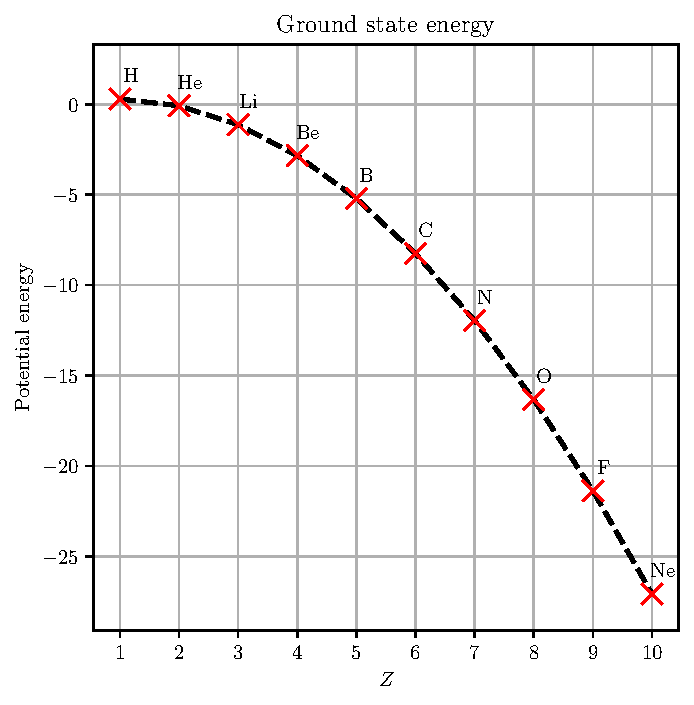
\includegraphics{figs/energy_plot.pdf}
    \caption{The expectation value of the ground states of an atom with two electrons as a function of the nuclear charge $Z$.\label{fig:energy}}
\end{figure}

Define the Hamiltonian in a second-quantized form and use this to compute the expectation value of the ground state (defining the so-called reference energy and later our Hartree-Fock functional) of
the helium atom.
Show that it is given by
\begin{equation}
    E[\Phi_0] = \expval{c}{\hat{H}}{c} = \sum_{i} \expval{i}{\hat{h}_0}{i} + \frac{1}{2} \sum_{ij} \left[\expval*{ij}{\frac{1}{r_{ij}}}{ij} - \expval*{ij}{\frac{1}{r_{ij}}}{ji}\right].
\end{equation}
Define properly the sums keeping in mind that the states $ij$ refer to all quantum numbers $n, l, m_l, s, m_s$.
Use the values for the various matrix elements listed at the end of the midterm to find the value of $E$ as function of $Z$ and compute $E$ as function of $Z$.

\subsection{}
We consider a Hamiltonian $\hat{H} = \hat{H}_0 + \hat{H}_I$, where $\hat{H}_0$ and $\hat{H}_I$ are one-electron and two-electron parts respectively, defined by
\begin{align}
    \hat{H}_0 &= \sum_{p q} \expval{p}{\hat{h}_0}{q} a_p^\dagger a_q, &
    \hat{H}_I &= \frac{1}{4} \sum_{pqrs} \expval{pq}{\hat{v}}{rs}_{AS} a_p^\dagger a_q^\dagger a_s a_r.
\end{align}

We have the normal-ordered form of annihilation and creation operators, relative to the reference state, where all creation operators are to the left of all annihilation operators.
For example, we have $N[a_p^\dagger a_q] = a_p^\dagger a_q$, $N[a_p a_q^\dagger] = -a_q^\dagger a_p$, where the sign is dependent on the number of permutations required to bring the operators to normal order.
We are interested in this, as
\begin{equation*}
    \expval{c}{N[A B\dotsm]}{c} = 0
\end{equation*}
if $N[A B \dotsm]$ is not empty, where $A, B, \dotsc$ are annihilation or creation operators.

With this, we have the contractions of operators, defined as
\begin{equation*}
    \wick{\c A \c B} = AB - N[AB].
\end{equation*}
Relative to our reference state, we have that
\begin{align*}
    \wick{\c a_i^\dagger \c a_j} &= \delta_{i j}, &
    \wick{\c a_a \c a_b^\dagger} &= \delta_{a b}
\end{align*}
are the only non-zero contractions.

For the one-body term, we then have
\begin{equation}
    \expval{c}{\hat{H}_0}{c} = \sum_{pq} \expval{p}{\hat{h}_0}{q} \expval{c}{a_p^\dagger a_q}{c} = \sum_{ij} \expval{i}{\hat{h}_0}{j} \delta_{ij} = \sum_{i} \expval{i}{\hat{h}_0}{i}.
\end{equation}

For the two-body term, writing $\ket{c} = \ket{i j}$ we first need to examine the possible contractions of $ i j p^\dagger q^\dagger s r j^\dagger i^\dagger$ and the resulting matrix element $\expval{pq}{V}{rs}_{AS}$.
We have
\begin{align*}
    \wick{
        \c2 j
        \c1 i
        \c1 p^\dagger
        \c2 q^\dagger
        \c2 s
        \c1 r
        \c1 i^\dagger
        \c2 j^\dagger
    } &= \delta_{jq} \delta_{ip} \delta_{sj} \delta_{ri} \to \expval{ij}{V}{ij}_{AS}, \\
    \wick{
        \c2 j
        \c1 i
        \c1 p^\dagger
        \c2 q^\dagger
        \c2 s
        \c1 r
        \c2 i^\dagger
        \c1 j^\dagger
    } &= -\delta_{jq} \delta_{ip} \delta_{si} \delta_{rj} \to -\expval{ij}{V}{ji}_{AS}, \\
    \wick{
        \c2 j
        \c1 i
        \c2 p^\dagger
        \c1 q^\dagger
        \c2 s
        \c1 r
        \c2 i^\dagger
        \c1 j^\dagger
    } &= \delta_{jp} \delta_{iq} \delta_{si} \delta_{rj} \to \expval{ji}{V}{ji}_{AS}, \\
    \wick{
        \c2 j
        \c1 i
        \c2 p^\dagger
        \c1 q^\dagger
        \c2 s
        \c1 r
        \c1 i^\dagger
        \c2 j^\dagger
    } &= -\delta_{jp} \delta_{iq} \delta_{sj} \delta_{ri} \to -\expval{ji}{V}{ij}_{AS}.
\end{align*}
As $\expval{\alpha \beta}{V}{\gamma \delta}_{AS} = - \expval{\alpha \beta}{V}{\delta \gamma}_{AS}$ we gather these terms, and inserting for $V$, leaving us with
\begin{equation}
    \expval{c}{\hat{H}_I}{c} = \frac{1}{2} \sum_{ij} \expval{ij}{\frac{1}{r_{ij}}}{ij}_{AS} = \frac{1}{2} \sum_{ij} \expval{ij}{\frac{1}{r_{ij}}}{ij} - \expval{ij}{\frac{1}{r_{ij}}}{ji}.
\end{equation}

Combining this with the one-body term, we have the total reference energy
\begin{equation}
    E[\Phi_0] = \expval{c}{\hat{H}}{c} = \sum_{i} \expval{i}{\hat{h}_0}{i} + \frac{1}{2} \sum_{ij} \expval{ij}{\frac{1}{r_{ij}}}{ij} - \expval{ij}{\frac{1}{r_{ij}}}{ji},
\end{equation}
as we wanted to show.

In the case of the electrons in the helium atom, we only have $n = 1$, $l = 0$, differing only in the spin quantum number $m_s = \pm 1/2$.
The expectation value of the one-body part is then
\begin{equation*}
    \expval{\Phi_0}{\hat{H}_0}{\Phi_0} = \sum_{\sigma \in \{\pm 1/2\}} \expval{1\sigma}{\hat{h}_0}{1\sigma} = -Z^2,
\end{equation*}
and the expectation value of the two-body part is, writing just $\sigma_{+}$ and $\sigma_{-}$ for the spins with $n = 1$,
\begin{equation*}
    \expval{\Phi_0}{\hat{H}_I}{\Phi_0}
    = \frac{1}{2} \sum_{\substack{\sigma_{+}\sigma_{-}\\ \sigma_{+} \neq \sigma_{-}}}
    \underbrace{\expval*{\sigma_{+} \sigma_{-}}{\frac{1}{r_{\sigma_{+}\sigma_{-}}}}{\sigma_{+} \sigma_{-}}}_{\textnormal{Direct term}}
    - \underbrace{\expval*{\sigma_{+} \sigma_{-}}{\frac{1}{r_{\sigma_{+}\sigma_{-}}}}{\sigma_{-}\sigma_{+}}}_{\textnormal{Exchange term}}.
\end{equation*}
The exchange term vanishes since the states are orthogonal, and we are left with the direct term.
We are then just left with
\begin{equation*}
    \expval{\Phi_0}{\hat{H}_I}{\Phi_0} = \frac{1}{2}\left[ \expval*{\sigma_{+} \sigma_{-}}{\frac{1}{r_{\sigma_{+} \sigma_{-}}}}{\sigma_{+} \sigma_{-}} + \expval*{\sigma_{-} \sigma_{+}}{\frac{1}{r_{\sigma_{+} \sigma_{-}}}}{\sigma_{-} \sigma_{+}}\right].
\end{equation*}
As $\hat{H}_I$ is invariant under the change of label $\sigma$, we can simplify this to
\begin{equation*}
    \expval{\Phi_0}{\hat{H}_I}{\Phi_0} = \expval*{\sigma_{+} \sigma_{-}}{\frac{1}{r_{\sigma_{+} \sigma_{-}}}}{\sigma_{+} \sigma_{-}} = \frac{5}{8} Z.
\end{equation*}

Combining this, we find that the expectation value of the ground state is
\begin{equation}
    E[\Phi_0] = -Z^2 + \tfrac{5}{8}Z,
\end{equation}
which as a function of $Z$ is shown in \autoref{fig:energy}.
For $Z = 2$, we find that
\begin{equation}
    E[\Phi_0] = -2.75 = -74.8 \ \text{eV}.
\end{equation}

\begin{figure}[ht]
    \centering
    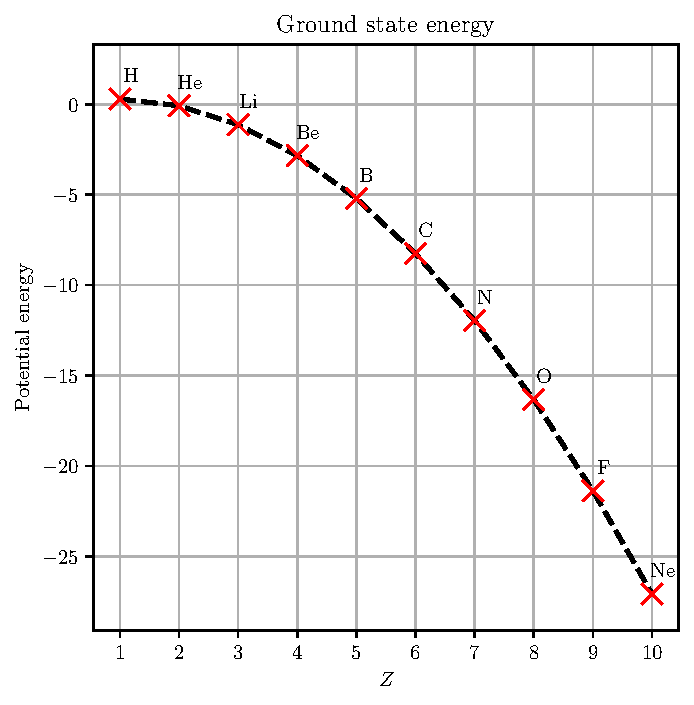
\includegraphics{figs/energy_plot.pdf}
    \caption{The expectation value of the ground states of an atom with two electrons as a function of the nuclear charge $Z$.\label{fig:energy}}
\end{figure}

\section{Limiting ourselves to one-particle-one excitations}
Hereafter we will limit ourselves to a system which now contains only one-particle-one-hole excitations beyond the chosen state $\ket{c}$.
Using the possible Slater determinants from exercise a) for the helium atom, find the expressions (without inserting the explicit values for the matrix elements first) for % chktex 10 % tex-fmt: skip
\begin{equation*}
    \expval{c}{\hat{H}}{\Phi_i^a},
\end{equation*}
and
\begin{equation*}
    \expval{\Phi_i^a}{\hat{H}}{\Phi_j^b}.
\end{equation*}
Represent these expressions in a diagrammatic form, both for the onebody part and the two-body part of the Hamiltonian.

Insert then the explicit values for the various matrix elements and set up the final Hamiltonian matrix and diagonalize it using for example Python as programming language.
Compare your results from those of exercise b) and comment your results. % chktex 10 % tex-fmt: skip

The exact energy with our Hamiltonian is $-2.9037$ atomic units for helium.
This value is also close to the experimental energy.

\subsection{}
In order to be able to handle the more complicated systems, we partition the Hamiltonian into
\begin{equation}
    \hat{H} = \underbrace{\mathcal{E}_0^{\text{ref}}}_{\expval{c}{\hat{H}_0}{c}} + \hat{F}_N + \hat{V}_N,
\end{equation}
where
\begin{align*}
    \hat{F}_N &= \sum_{pq} \expval{p}{f}{q} \{a_p^\dagger a_q\}, \qquad
    \expval{p}{f}{q} = \expval{p}{\hat{h}_0}{q} + \sum_{i} \expval{pi}{V}{qi}_{AS}, \\
    \hat{V}_N &= \frac{1}{4} \sum_{pqrs} \expval{pq}{V}{rs}_{AS} \{a_p^\dagger a_q^\dagger a_s a_r\}.
\end{align*}

Considering then $\expval{c}{\hat{H}}{\Phi_i^a}$, we firstly have $\expval{c}{\mathcal{E}_0^{\text{Ref}}}{\Phi_i^a} = 0$, as $\braket{c}{\Phi_i^a} = 0$.
For the next term, we have
\begin{align*}
    \expval{c}{\hat{F}_N}{\Phi_i^a} &= \sum_{pq} \expval{p}{f}{q} \expval{c}{\{ a_p^\dagger a_q \}}{\Phi_i^a}
    = \sum_{pq} \expval{p}{f}{q} \wick{
        \langle c \vert
        \{ \c2 a_p^\dagger \c1 a_q \}
        \{ \c1 a_a^\dagger \c2 a_i \}
        \vert c \rangle
    } \\
    &= \sum_{pq} \expval{p}{f}{q} \delta_{pi} \delta_{qa}
    = \expval{i}{f}{a} \\
    &= \expval{i}{\hat{h}_0}{a} + \sum_{j} \expval{ij}{V}{aj}_{AS}.
\end{align*}
For the last term, we get
\begin{align*}
    \expval{c}{\hat{V}_N}{\Phi_i^a} &= \frac{1}{4} \sum_{pqrs} \expval{pq}{V}{rs}_{AS} \expval{c}{\{a_p^\dagger a_q^\dagger a_s a_r \}}{\Phi_i^a} \\
    &= \frac{1}{4} \sum_{pqrs} \expval{pq}{V}{rs}_{AS} \wick{
        \langle c \vert
        \{ a_p^\dagger a_q^\dagger a_s a_r \}
        \{ a_a^\dagger a_i \}
        \vert c \rangle
    } \\
    &= 0,
\end{align*}
which vanishes as this would require a contraction within the normal ordered operator $\{a_p^\dagger a_q^\dagger a_s a_r\}$.

Considering next $\expval{\Phi_i^a}{\hat{H}}{\Phi_{j}^{b}}$, we have
\begin{equation*}
    \expval{\Phi_i^a}{\mathcal{E}_0^{\text{Ref}}}{\Phi_{j}^{b}} = \mathcal{E}_0^{\text{Ref}}
    \expval{c}{\wick{
            \{ \c2 a_i^\dagger \c1 a_a \}
            \{ \c1 a_b^\dagger \c2 a_j \}
        }
    }{c}
    = \delta_{ij} \delta_{ab} \mathcal{E}_0^{\text{Ref}}.
\end{equation*}
Next, we have
\begin{align*}
    \expval{\Phi_i^a}{\hat{F}_N}{\Phi_{j}^{b}}
    &= \sum_{pq} \expval{p}{f}{q} \expval{\Phi_i^a}{\{ a_p^\dagger a_q \}}{\Phi_{j}^{b}} \\
    &= \sum_{pq}
    \expval{p}{f}{q}
    \expval{c}{
        \wick{
            \{ a_i^\dagger a_a \}
            \{ a_p^\dagger a_q \}
            \{ a_b^\dagger a_j \}
        }
    }{c}.
\end{align*}
Considering the contractions seperately, we have the two possible contractions
\begin{align*}
    \wick{
        \langle c \vert
        \{ \c2 a_i^\dagger \c1 a_a \}
        \{ \c1 a_p^\dagger \c1 a_q \}
        \{ \c1 a_b^\dagger \c2 a_j \}
        \vert c \rangle
    }
    &= \delta_{ij} \delta_{ap} \delta_{bq}, \\
    \wick{
        \langle c \vert
        \{ \c1 a_i^\dagger \c2 a_a \}
        \{ \c3 a_p^\dagger \c1 a_q \}
        \{ \c2 a_b^\dagger \c3 a_j \}
        \vert c \rangle
    } &= -\delta_{iq} \delta_{ab} \delta_{jp},
\end{align*}
leaving us with
\begin{equation*}
    \expval{\Phi_i^a}{\hat{F}_N}{\Phi_{j}^{b}} = \expval{a}{f}{b} \delta_{ij} - \expval{j}{f}{i} \delta_{ab}.
\end{equation*}
Finally, considering the last term, we have
\begin{align*}
    \expval{\Phi_i^a}{\hat{V}_N}{\Phi_{j}^{b}}
    &= \frac{1}{4} \sum_{pqrs} \expval{pq}{V}{rs}_{AS} \expval{\Phi_i^a}{\{a_p^\dagger a_q^\dagger a_s a_r\}}{\Phi_{j}^{b}} \\
    &= \frac{1}{4} \sum_{pqrs} \expval{pq}{V}{rs}_{AS} \expval{c}{
        \wick{
            \{ a_i^\dagger a_a \}
            \{ a_p^\dagger a_q^\dagger a_s a_r \}
            \{ a_b^\dagger a_j \}
        }
    }{c}.
\end{align*}
Considering the contractions seperately, we have the four possible contractions
\begin{align*}
    \wick{
        \langle c \vert
        \{ \c2 a_i^\dagger \c1 a_a \}
        \{ \c1 a_p^\dagger \c3 a_q^\dagger \c2 a_s \c1 a_r \}
        \{ \c1 a_b^\dagger \c3 a_j \}
        \vert c \rangle
    }
    &= -\delta_{is} \delta_{ap} \delta_{jq} \delta_{br}, \\
    \wick{
        \langle c \vert
        \{ \c2 a_i^\dagger \c1 a_a \}
        \{ \c3 a_p^\dagger \c1 a_q^\dagger \c2 a_s \c1 a_r \}
        \{ \c1 a_b^\dagger \c3 a_j \}
        \vert c \rangle
    } &= \delta_{is} \delta_{aq} \delta_{jp} \delta_{br}, \\
    \wick{
        \langle c \vert
        \{ \c2 a_i^\dagger \c1 a_a \}
        \{ \c1 a_p^\dagger \c3 a_q^\dagger \c1 a_s \c2 a_r \}
        \{ \c1 a_b^\dagger \c3 a_j \}
        \vert c \rangle
    } &= \delta_{ir} \delta_{ap} \delta_{jq} \delta_{bs}, \\
    \wick{
        \langle c \vert
        \{ \c2 a_i^\dagger \c1 a_a \}
        \{ \c3 a_p^\dagger \c1 a_q^\dagger \c1 a_s \c2 a_r \}
        \{ \c1 a_b^\dagger \c3 a_j \}
        \vert c \rangle
    } &= -\delta_{ir} \delta_{aq} \delta_{jp} \delta_{bs}.
\end{align*}
Any contraction between $\{a_i^\dagger a_a\}$ and $\{a_b^\dagger a_j\}$ will vanish, as this would require a contraction within central normal ordered operator.
This leaves us with
\begin{align*}
    \expval{\Phi_i^a}{\hat{V}_N}{\Phi_{j}^{b}}
    &= \frac{1}{4} \sum_{pqrs} \expval{pq}{V}{rs}_{AS} \\
    &\times \Big[
        - \delta_{is} \delta_{ap} \delta_{jq} \delta_{br}
        + \delta_{is} \delta_{aq} \delta_{jp} \delta_{br}
        + \delta_{ir} \delta_{ap} \delta_{jq} \delta_{bs}
        - \delta_{ir} \delta_{aq} \delta_{jp} \delta_{bs}
    \Big],
\end{align*}
which when inserted gives
\begin{align*}
    \expval{\Phi_i^a}{\hat{V}_N}{\Phi_{j}^{b}} &= \frac{1}{4} \big[
        -\expval{aj}{V}{bi}_{AS} + \expval{ja}{V}{bi}_{AS} + \expval{aj}{V}{ib}_{AS} - \expval{ja}{V}{ib}_{AS}
    \big] \\
    &= \frac{1}{4} \big[
        \expval{aj}{V}{ib}_{AS} + \expval{ja}{V}{bi}_{AS} + \expval{aj}{V}{ib}_{AS} + \expval{ja}{V}{bi}_{AS}
    \big] \\
    &= \expval{aj}{V}{ib}_{AS}.
\end{align*}
We have thus shown that
\begin{equation}
    \begin{split}
        \expval{c}{\hat{H}}{\Phi_i^a} &= \expval{i}{\hat{h}_0}{a} + \sum_{j} \expval{ij}{V}{aj}_{AS} \\
        \expval{\Phi_i^a}{\hat{H}}{\Phi_{j}^{b}} &= \delta_{ij} \delta_{ab} \mathcal{E}_0^{\text{Ref}} + \expval{a}{f}{b} \delta_{ij} - \expval{j}{f}{i} \delta_{ab} + \expval{aj}{V}{ib}_{AS}.
    \end{split}
\end{equation}
% Inserting for $f$, we can simplify the later expressions, as $\hat{h}_0$ defined in Eq.~\eqref{eq:onebody} contains a $\delta_{\alpha \beta}$.
% We then have
% \begin{equation*}
%     \expval{\alpha}{f}{\beta} = \expval{\alpha}{\hat{h}_0}{\beta} + \sum_{k} \expval{\alpha k}{V}{\beta k}_{AS} = \delta_{\alpha \beta} \expval{\alpha}{\hat{h}_0}{\alpha} + \sum_{k} \expval{\alpha k}{V}{\beta k}_{AS}.
% \end{equation*}
% Our final expression for $\expval{\Phi_i^a}{\hat{H}}{\Phi_{j}^{b}}$ then becomes
% \begin{align*}
%     \expval{\Phi_i^a}{\hat{H}}{\Phi_{j}^{b}} &= \delta_{ij} \delta_{ab} \Big[ \mathcal{E}_0^{\text{Ref}} + \expval{a}{\hat{h}_0}{a}  - \expval{i}{\hat{h}_0}{i} \Big] + \expval{aj}{V}{ib}_{AS} \\
%     &+ \sum_{k} \Big[ \delta_{ij} \expval{ak}{V}{bk} - \delta_{ab} \expval{jk}{V}{ik} \Big]
% \end{align*}

% Considering the different cases of $(i, a), (j, b)$ for the helium atom, we have when $i = j$ and $a = b$
% \begin{align*}
%     \expval{\Phi_i^a}{\hat{H}}{\Phi_i^a} &= \mathcal{E}_0^{\text{Ref}} + \expval{a}{\hat{h}_0}{a} - \expval{i}{\hat{h}_0}{i} + \expval{ai}{V}{ia}_{AS}  \\
%     &+ \sum_{k} \Big[ \expval{ak}{V}{ak}_{AS} - \expval{ik}{V}{ik}_{AS} \Big],
% \end{align*}
% When $i = j$ and $a \neq b$
% \begin{equation*}
%     \expval{\Phi_i^a}{\hat{H}}{\Phi_i^b} = \expval{ai}{V}{ib}_{AS} + \sum_k \Big[ \expval{ak}{V}{bk}_{AS} \Big],
% \end{equation*}
% When $i \neq j$ and $a = b$
% \begin{equation*}
%     \expval{\Phi_i^a}{\hat{H}}{\Phi_j^a} = \expval{aj}{V}{ia}_{AS} - \sum_k \Big[ \expval{jk}{V}{ik}_{AS} \Big],
% \end{equation*}
% and finally when $i \neq j$ and $a \neq b$
% \begin{equation*}
%     \expval{\Phi_i^a}{\hat{H}}{\Phi_j^b} = \expval{aj}{V}{ib}_{AS}.
% \end{equation*}

Inserting for the explicit matrix elements, we get that the energy with our Hamiltonian is $-2.8386$ atomic units, or $-77.2112 \ \text{eV}$ for the helium atom.
We see that we have a higher value than the exact energy, which is expected as the true energy serves as a lower bound to the truncated Hamiltonian.
We also see an improvement from our previous results, which stem from the fact that we are truncating at a higher level of excitations.
The energy is computed with the code in \verb|src/get_energy.py|.


\section{Moving to the Beryllium atom}
We switch now to approximative methods, in our case Hartree-Fock theory and many-body perturbation theory.
Hereafter we will define our model space to consist of the single-particle levels $p = 1, 2$.
The remaining levels $p = 3, 4$ define our excluded space.
This means that our ground state Slater determinant consists of four particles which can be placed in the doubly degenerate orbits $p = 1$ and $p = 2$.
Our first step is to perform a Hartree-Fock calculation with the pairing Hamiltonian.
Write first the normal-ordered Hamiltonian with respect to the above reference state given by four spin $1/2$ fermions in the single-particle levels $p = 1, 2$.
Write down the normal-ordered Hamiltonian and set up the standard Hartree-Fock equations for the above system (often called restricted Hartree-Fock due to the fact that  we have an equal number of spin-orbitals).
These equations are sometimes also called the canonical Hartree-Fock equations.
They are the same as those that we discussed earlier.
This means that we have a Hartree-Fock Hamiltonian $\hat{h}^{\mathrm{HF}} \vert p \rangle = \epsilon^{\mathrm{HF}} \vert p \rangle$, where $p$ are both hole and particle states.

\subsection{}
We begin by writing the normal-ordered form of the single-particle term of the Hamiltonian with respect to the reference state $\ket{\Phi_0}$,
\begin{equation*}
    \hat{H}_0 = \sum_{p\sigma} (p-1) a_{p\sigma}^\dagger a_{p\sigma}.
\end{equation*}
We have that
\begin{align*}
    \hat{H}_0 &= \langle \Phi_0 | \hat{H}_0 | \Phi_0 \rangle + \hat{H}_0^N \\
    \sum_{p\sigma} (p-1) a_{p\sigma}^\dagger a_{p\sigma} &= \langle \Phi_0 | \hat{H}_0 | \Phi_0 \rangle + \sum_{p\sigma} (p-1) \{ a_{p\sigma}^\dagger a_{p\sigma} \}.
\end{align*}
Next, we have the two-body term of the Hamiltonian,
\begin{equation*}
    \hat{V} = -\frac{1}{2} g \sum_{pq} a^{\dagger}_{p+} a^{\dagger}_{p-} a_{q-} a_{q+}.
\end{equation*}

For the annihilation and creation operators in the two-body term, we have the possible contractions
\begin{align*}
    \wick{
        \c1 a_{p+}^\dagger
        a_{p-}^\dagger
        a_{q-}
        \c1 a_{q+}
    } & = \delta_{pq} n_{p+} a_{p-}^\dagger a_{q-}, \\%[0.5em]
    \wick{
        a_{p+}^\dagger
        \c1 a_{p-}^\dagger
        \c1 a_{q-}
        a_{q+}
    } & = \delta_{pq} n_{p-} a_{p+}^\dagger a_{q+}, \\%[0.5em]
    \wick{
        \c2 a_{p+}^\dagger
        \c1 a_{p-}^\dagger
        \c1 a_{q-}
        \c2 a_{q+}
    } & = \delta_{pq} n_{p+} n_{p-} a_{p+}^\dagger a_{q+} a_{p-}^\dagger a_{q-},
\end{align*}
where $n_{p\sigma} = 1$ if $p = 1, 2$ and $n_{p\sigma} = 0$ otherwise.
Note that as we have terms $n_{p\pm} a_{p\mp}^\dagger a_{p\mp}$, we only get contributions when both spins at a given level is occupied, i.e., from unbroken pairs.

We switch now to particle-hole formalism, where we denote states below the Fermi level as $i, j, \ldots \in \{1, 2\}$, states above the Fermi level as $a, b, \ldots \in \{3, 4\}$, and unrestricted indices as $p, q, \ldots$.
The normal-ordered form of the two-body term is then
\begin{align*}
    \hat{V} =& -\frac{1}{2} g \sum_{pq} \{ a_{p+}^\dagger a_{p-}^\dagger a_{q-} a_{q+} \}
    -\frac{1}{2} g \sum_{i} \left[ a_{p-}^\dagger a_{p-} + a_{p+}^\dagger a_{p+} \right] \\
    &- \frac{1}{2} g \sum_{i} 1 \\
    =& -\frac{1}{2} g \sum_{pq} \{ a_{p+}^\dagger a_{p-}^\dagger a_{q-} a_{q+} \}
    -\frac{1}{2} g \sum_{i \sigma} a_{i\sigma}^\dagger a_{i\sigma}- g.
\end{align*}

Grouping the terms of parts involving no particles, one particle, and two particles respectively, we have the normal-ordered Hamiltonian as
\begin{equation*}
    \hat{H} = E_0^{\text{Ref}} + \hat{H}_0^N + \hat{V}^N,
\end{equation*}
where
\begin{align*}
    E_0^{\text{Ref}} &= 2 - g \\
    \hat{H}_0^N &= \sum_{p\sigma} (p-1) \{ a_{p\sigma}^\dagger a_{p\sigma} \} - \frac{1}{2} g \sum_{i \sigma} \{ a_{i\sigma}^\dagger a_{i\sigma} \} \\
    \hat{V}^N &= -\frac{1}{2} g \sum_{pq} \{ a_{p+}^\dagger a_{p-}^\dagger a_{q-} a_{q+} \}.
\end{align*}

We begin by defining the single-particle operator $\hat{f}$, which in the general case is given by
\begin{equation*}
    \langle p \vert \hat{f} \vert q \rangle = \langle p \vert \hat{H}_0 \vert q \rangle + \sum_{j} \langle p j \vert \hat{V} \vert q j \rangle.
\end{equation*}
For our case, we have that
\begin{align*}
    \langle p \vert \hat{f} \vert q \rangle &= (p-1) \delta_{pq} - \frac{1}{2} g \sum_{j} \langle p j \vert \hat{V} \vert q j \rangle \\
    &= (p-1) \delta_{pq} - \frac{1}{2} g \sum_{j} \langle p j \vert \hat{V} \vert q j \rangle \\
    &= (p-1) \delta_{pq} - \frac{1}{2} g \sum_{j} \langle p j \vert \hat{V} \vert q j \rangle.
\end{align*}



\section{Hartree-Fock}
\subsection*{Preamble}
With a given energy functional, we can perform at least two types of variational strategies.
These are:
\begin{enumerate}
    \item Vary the Slater determinant by changing the spatial part of the single-particle wave functions themselves, or

    \item Expand the single-particle functions in a known basis  and vary the coefficients, that is, the new function single-particle wave function $\ket{p}$ is written as a linear expansion in terms of a fixed basis $\phi$ (harmonic oscillator, Laguerre polynomials etc)
        \begin{equation*}
            \psi_p  = \sum_{\lambda} C_{p\lambda}\phi_{\lambda}
        \end{equation*}
\end{enumerate}
Both cases lead to a new Slater determinant which is related to the previous via a unitary transformation.
Below we will set up the Hartree-Fock equations using the second option.
We assume that our basis is still formed by the hydrogen-like wave functions.
We consider a Slater determinant built up of single-particle orbitals $\phi_{\lambda}$ where the indices $\lambda$ refer to specific single-particle states.
As an example, you could think of the ground state ansatz for the beryllium atom.

The unitary transformation
\begin{equation*}
    \psi_p  = \sum_{\lambda} C_{p\lambda}\phi_{\lambda},
\end{equation*}
brings us into the new basis $\psi$.
The new basis is orthonormal and $C$ is a unitary matrix.

\subsection*{Problem definition}
Minimizing with respect to $C^*_{p\alpha}$, remembering that $C^*_{p\alpha}$ and $C_{p\alpha}$ (and that the indices contain all single-particle quantum numbers including spin) are independent and defining
\begin{equation*}
    h_{\alpha\gamma}^\HF = \expval{\alpha}{h}{\gamma} + \sum_{p} \sum_{\beta\delta} C^*_{p\beta} C_{p\delta} \expval{\alpha\beta}{V}{\gamma\delta}_{AS},
\end{equation*}
show that you can write the Hartree-Fock equations as
\begin{equation*}
    \sum_{\gamma} h_{\alpha\gamma}^\HF C_{p\gamma} = \epsilon_p^{\mathrm{HF}} C_{p\alpha}. \label{eq:newhf}
\end{equation*}

Explain the meaning of the different terms and define the Hartree-Fock operator in second quantization.
Write down its diagrammatic representation as well.
The greek letters refer to the wave functions in the original basis (in our case the hydrogen-like wave functions) while roman letters refer to the new basis.

\subsection{}
We previously defined the energy functional as, using greek indices for the original basis,
\begin{equation*}
    E[\Phi] = \expval{\Phi}{\hat{H}}{\Phi} = \sum_{\alpha} \expval{\alpha}{\hat{h}_0}{\alpha} + \frac{1}{2} \sum_{\alpha\beta} \expval{\alpha\beta}{\hat{v}}{\alpha \beta}_{AS}.
\end{equation*}
In the new basis, we have
\begin{equation*}
    E[\Phi^\HF] = \sum_{i} \expval{i}{\hat{h}_0}{i} + \frac{1}{2} \sum_{ij} \expval{ij}{\hat{v}}{ij}_{AS}.
\end{equation*}
As $\ket{i} = \sum_{\alpha} C_{i \alpha} \ket{\alpha}$, we also have
\begin{equation*}
    \bra{i} = \ket{i}^\dagger
    = \left[ \sum_{\alpha} C_{i \alpha} \ket{\alpha} \right]^\dagger
    = \sum_{\alpha} C_{i \alpha}^* \bra{\alpha}.
\end{equation*}
This means that we can rewrite the one-body as
\begin{align*}
    \sum_i \expval{i}{h}{i} = \sum_{i} \sum_{\alpha\beta} \expval{\alpha}{C_{i \alpha}^* h C_{i \beta}}{\beta} = \sum_{i} \sum_{\alpha\beta} C_{i \alpha}^* C_{i \beta}  \expval{\alpha}{h}{\beta}.
\end{align*}
Similarly, we get the two-body part as
\begin{equation*}
    \frac{1}{2} \sum_{ij} \expval{ij}{v}{ij}_{AS} = \frac{1}{2} \sum_{ij} \sum_{\alpha\beta\gamma\delta} C_{i \alpha}^* C_{j \beta}^* C_{i \gamma} C_{j \delta} \expval{\alpha\beta}{v}{\gamma\delta}_{AS}.
\end{equation*}
Defining this as a functional of the coefficients $C$, we have
\begin{equation}\label{eq:E0}
    E_0[C] = \sum_{i} \sum_{\alpha\beta} C_{i \alpha}^* C_{i \beta}  \expval{\alpha}{h}{\beta} + \frac{1}{2} \sum_{ij} \sum_{\alpha\beta\gamma\delta} C_{i \alpha}^* C_{j \beta}^* C_{i \gamma} C_{j \delta} \expval{\alpha\beta}{v}{\gamma\delta}_{AS}.
\end{equation}

As we are working with orthonormal basis functions, we have
\begin{equation*}
    \braket{i}{j} = \delta_{ij} = \sum_{\alpha\beta} C_{i \alpha}^* C_{i \beta} \braket{\alpha}{\beta} = \sum_{\alpha} C_{i \alpha}^* C_{i \alpha}.
\end{equation*}
With this, we define a functional $F[C]$ as
\begin{equation*}
    F[C] = E_0[C] - \sum_{i} \lambda_i \sum_{\alpha} C_{i \alpha}^* C_{i \alpha},
\end{equation*}
where $\lambda_i$ are the Lagrange multipliers enforcing the orthonormality of the basis functions and $N$ is the number of states.

Minimizing $F$ with respect to $C^*_{p\alpha}$, we wish to solve
\begin{equation*}
    \frac{\diff F}{\diff C^*_{p\alpha}}[C] = \frac{\diff}{\diff C_{i \alpha}^*} \left[ E_0[C] - \sum_j \lambda_j \sum_{\alpha} C_{j \alpha}^* C_{j \alpha} \right] = 0.
\end{equation*}
Considering the one-body part of $E_0$, we have
\begin{equation*}
    \frac{\diff}{\diff C_{i \alpha}^*} \sum_{i} \sum_{\alpha\beta} C_{i \alpha}^* C_{i \beta}  \expval{\alpha}{h}{\beta} = \sum_{\beta} C_{i \beta} \expval{\alpha}{h}{\beta}.
\end{equation*}
For the two-body part, we firstly note that $C_{i \alpha}^*$ and $C_{j \beta}^*$ of Eq.~\eqref{eq:E0} are dummy indices, meaning the factor of $1/2$ gets canceled out.
This gives us
\begin{equation*}
    \frac{\diff}{\diff C_{i \alpha}^*} \frac{1}{2} \sum_{ij} \sum_{\alpha\beta\gamma\delta} C_{i \alpha}^* C_{j \beta}^* C_{i \gamma} C_{j \delta} \expval{\alpha\beta}{v}{\gamma\delta}_{AS} = \sum_j \sum_{\beta\gamma\delta} C_{j \beta}^* C_{i \gamma} C_{j \delta} \expval{\alpha\beta}{v}{\gamma\delta}_{AS}.
\end{equation*}
For the term enforcing orthonormality, we have simply
\begin{equation*}
    \frac{\diff}{\diff C_{i \alpha}^*} \sum_{i} \lambda_i \sum_{\alpha} C_{i \alpha}^* C_{i \alpha} = \lambda_i C_{i \alpha}.
\end{equation*}
Combining these terms, we have
\begin{equation*}
    \sum_{\beta} C_{i \beta} \expval{\alpha}{h}{\beta} + \sum_j \sum_{\beta\gamma\delta} C_{j \beta}^* C_{i \gamma} C_{j \delta} \expval{\alpha\beta}{v}{\gamma\delta}_{AS} - \lambda_i C_{i \alpha} = 0.
\end{equation*}
Recognizing $\lambda_i$ as the eigenvalues $\varepsilon_i^\HF$, we can rewrite this as
\begin{equation*}
    \sum_{\beta} C_{i \beta} \expval{\alpha}{h}{\beta} + \sum_j \sum_{\beta\gamma\delta} C_{j \beta}^* C_{i \gamma} C_{j \delta} \expval{\alpha\beta}{v}{\gamma\delta}_{AS} = \varepsilon_i^\HF C_{i \alpha}.
\end{equation*}

Changing the label of the dummy variables $\beta \mapsto \gamma$ in the one-body term and $i \mapsto p$ everywhere, we can write this as
\begin{gather*}
    \sum_{\gamma} C_{p \gamma} \expval{\alpha}{h}{\gamma} + \sum_j \sum_{\beta\gamma\delta} C_{j \beta}^* C_{p \gamma} C_{j \delta} \expval{\alpha\beta}{v}{\gamma\delta}_{AS} = \varepsilon_p^\HF C_{p \alpha} \\
    \sum_{\gamma}  \left[ C_{p \gamma} \expval{\alpha}{h}{\gamma} + \sum_j \sum_{\beta\delta} C_{j \beta}^* C_{p \gamma} C_{j \delta} \expval{\alpha\beta}{v}{\gamma\delta}_{AS} \right] = \varepsilon_p^\HF C_{p \alpha} \\
    \sum_{\gamma} h_{\alpha\gamma}^\HF C_{p \gamma} = \varepsilon_p^\HF C_{p \alpha},
\end{gather*}
as we wanted to show.


\section{The Hartree-Fock matrices}
Diagram 1 in Fig.~\ref{fig:diagrams} represents a second-order contribution to the energy and a so-called $2p-2h$ contribution to the intermediate states.
Write down the expression for the wave operator in this case and compare the possible contributions with the configuration interaction calculations of exercise 3). % chktex 10 % tex-fmt: skip
Comment your results for various values of $g \in [-1,1]$.

\subsection{}
The second order wave operator is given by
\begin{equation*}
    \Psi^{(1)} = \frac{\hat{Q}}{\mathcal{E}_0 - \hat{H}_0} \hat{V} \vert \Phi_0 \rangle,
\end{equation*}


\end{document} % chktex 17
